An $n$-bit analog-to-digital converter functions --- at least at a high level --- by mapping a capped range of input voltages~(typically starting at zero and ending at some full-scale voltage~$V_\text{FS}$) into~$2^n$ discrete, non-intersecting values, sometimes labeled~$V_i$.  The output voltage is simply the largest discretized voltage that the input exceeds.  Because an analog input voltage is being represented by one of a finite set of discrete values, the index~$i$ of the corresponding output~$V_i$ can be expressed as a series of~$2^n$ binary bits.

When the input is a time-varying signal, the converter samples the input at a regular frequency~$f_s$, producing a new output as previously described for each sample.  An example of such a sampling and the digital output signal can be seen in Figure~\ref{fig:theory}.
%
\begin{figure}[H]
	\centering
	\subfloat[Analog input]{\label{fig:theoryAnalog}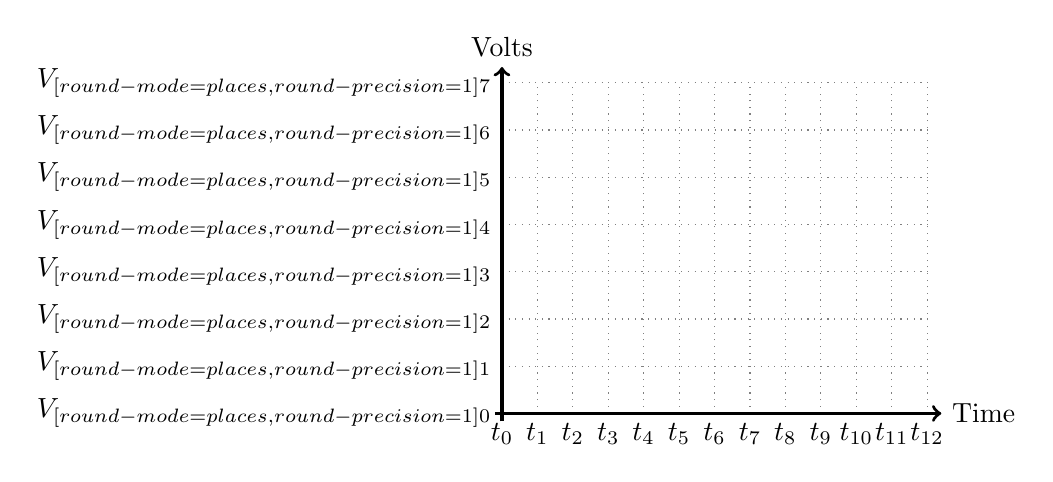
\begin{tikzpicture}[xscale=.9]
	% samples
	\draw[xstep=.5, ystep=.6, thin, color=gray, dotted] (0,0) grid (6, 4.2);

	% path
    \draw[thick] plot[id=sin,samples=1000,domain=0:6] function{-((x/2-1)**2)+4};

	% xtics
	\foreach \x in {0, ..., 12}
	{
		\draw ({\x/2}, 0) node[below] {$t_{\x}$};
	}

	% ytics
	\foreach \y in {0, 1, ..., 7.1}
	{
		\draw[thick] (0, .6*\y) node[left] {$V_{\num[round-mode=places, round-precision=1]{\y}}$};
	}

	% axes
    \draw[->, very thick] (-0.1,0) -- (6.2,0) node[right] {Time};
    \draw[->, very thick] (0,-.1) -- (0,4.4) node[above] {Volts};
\end{tikzpicture}
}
	\subfloat[Discrete output]{\label{fig:theoryDiscrete}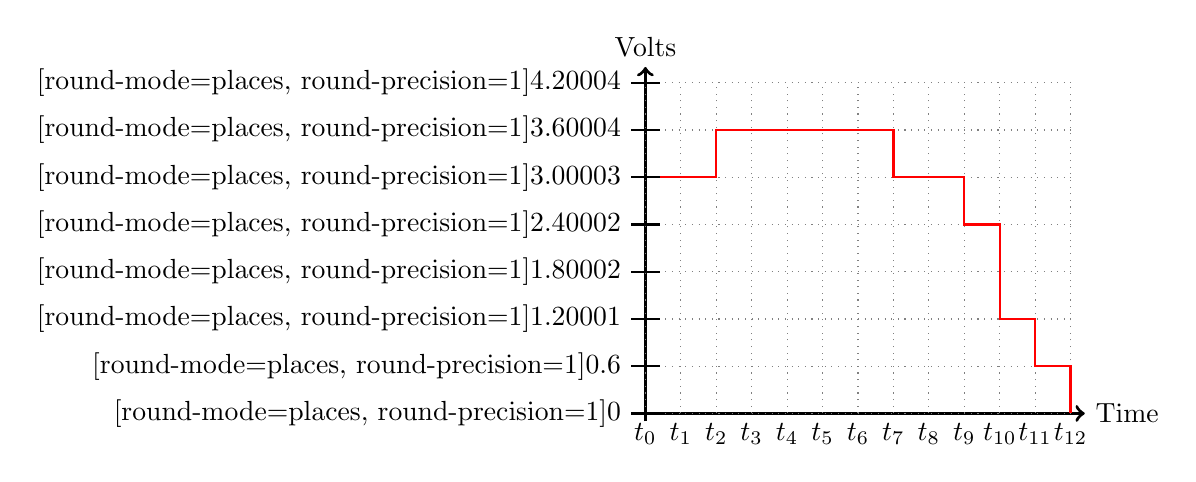
\begin{tikzpicture}[xscale=.9]
		% axes
    	\draw[->, very thick] (-0.1,0) -- (6.2,0) node[right] {Time};
    	\draw[->, very thick] (0,-.1) -- (0,4.4) node[above] {Volts};

		% samples
		\draw[xstep=.5, ystep=.6, thin, color=gray, dotted] (0,0) grid (6, 4.2);

		% discrete
		\draw[thick, color=red]
		(0, 3)
		-- (.5, 3) -- (1, 3)
		-- (1, 3.6) -- (1.5, 3.6) -- (2, 3.6) -- (2.5, 3.6) -- (3, 3.6) -- (3.5, 3.6)
		-- (3.5, 3) -- (4, 3) -- (4.5, 3)
		-- (4.5, 2.4) -- (5, 2.4)
		-- (5, 1.2) -- (5.5, 1.2)
		-- (5.5, 0.6) -- (6.0, 0.6)
		-- (6.0, 0);

		% xtics
		\foreach \x in {0, ..., 12}
		{
			\draw ({\x/2}, 0) node[below] {$t_{\x}$};
		}

		% ytics
		\foreach \y in {0, 0.6, ..., 4.3}
		{
			\draw[thick] (.2, \y) -- (-.2, \y) node[left] {\num[round-mode=places, round-precision=1]{\y}};
		}
\end{tikzpicture}
}

	\parbox{.8\textwidth}{
	\caption[Theory Plots]{Theoretical input and output for an analog-to-digital signal.  This is not a very accurate representation as the sampling frequency~$f_s$ and resolution are fairly large, leading to a loss of information.}
	\label{fig:theory}}
\end{figure}
%
While the digital output of this arbitrary signal resembles the input, it is clearly not very accurate.  This is a combined result of the resolution and sampling frequency being far too low.  An increased resolution~(here only 3-bits, or~$2^3 = 8$ possible values) would allow the maximum value of the signal located at~$t_4$ to be represented, eliminating the flat region between~$t_2$ and~$t_7$.  Likewise, increasing the sampling frequency would prevent a value from being skipped as~$V_3$ is at~$t_{10}$.

In order to simplify the process of using an ADC integrated circuit~(IC), a preconstructed circuit was provided to students~(the schematic for which is shown in Figure~\ref{fig:adcSchem}).
%
\begin{figure}[H]
	\centering
	\begin{circuitikz}
	\tikzstyle{leftPin}  = [anchor=west]
	\tikzstyle{rightPin} = [left]

	% body
	\draw[ultra thick] (-2, -4) rectangle (2, 4);

	% left pins

	% right pins
	\foreach \y in {7, ..., 0}
	{
		\draw (2, \y-3.5) node[rightPin] (b\y) {B\y}
		to [short] ++(.5,0) to [R, l=$R$] ++(1.5,0)
		++(1.5, 0) to [led, *-] ++(-1.5, 0);
	}

	\foreach \pin in {11,...,18}
	{
		\draw (2, 14.5-\pin) node[above right] {\pin};
	}

	\draw (b7) node[left=4pt] {MSB}
	(b0) node[left=4pt] {LSB};

	% 5V rail
	\draw (5.5, -3.5) to [short] ++(0, 8.5) node[above] {\SI{5.2}{\volt}};

	\draw (0, 4) node[above left] {20} to [short] ++(0, 2) coordinate (top junc) to [short] ++(1, 0)
	to [C, l=$C_4$: \SI{10}{\micro\farad}] ++(0, -1) node[ground] {}
	(top junc) to [short] ++(0, .5) node[above] {\SI{5.12}{\volt}};

	% left pins

\end{circuitikz}

	\parbox{.8\textwidth}{
	\caption[ADC Schematic]{Provided schematic for implenting an ADC0804 IC to construct a correctly-functioning analog-to-digital converter.  This system was available as a pre-assembled circuit.  As such, students were only responsible for operating the converter correctly.}
	\label{fig:adcSchem}}
\end{figure}
%
While this circuit looks daunting at first, there were primarily four things students were required to understand:  pin~6~($V_\text{IN}+$), pin~9~($V_\text{REF}$), pins~11 through~18~(the LED outputs), and pin~20~($V_\text{CC}$).

\begin{description}
	\item[Pin 6]{Pin six is the interface between the ADC and the input signal.  For this experiment it was either a DC voltage supply or a function generator.}

	\item[Pin 9]{The voltage at~$V_\text{REF}$ is used to determine the full-scale voltage, previously defined as~$V_\text{FS}$.  If left un-connected,~$V_\text{FS}$ defaults to~$V_\text{CC}$, or the ADC's drive voltage; if connected to a voltage source,~$V_\text{FS}$ is set to twice the voltage measured at pin nine.  This allows the circuit to be driven at a TTL-compliant~\SI{5}{\volt} while measuring voltages that are comparatively much lower, ensuring that the device does not turn off.}

	\item[Pins 11-18]{Pins eleven through eighteen represent the LED outputs of the system, used to display a binary value corresponding to the sampled input voltage~(where pin 11 is the least-significant bit.) The configuration of the LEDs is notable here, as they share a common~\SI{5}{\volt} source and are turned on by pulling the corresponding pin to ground.  While this is counter-intuitive as far as binary logic is concerned, it is necessary.  Had the LEDs been installed with a common ground in place of the~\SI{5}{\volt} source, the ADC IC would not be able to source enough current~(roughly~\SI{40}{\milli\ampere}) for the case that all LEDs would be on.  By using the IC to sink said current, all devices will remain undamaged.}

	\item[Pin 20]{Pin twenty is the source voltage~$V_\text{CC}$ of the entire system, used to drive both the IC and the LEDs.  It was tuned in-lab for the given experiment to ensure that all elements function properly.}
\end{description}
